% Chapter 1

\chapter{Resultados} % Main chapter title

\label{Cap_Res} % For referencing the chapter elsewhere, use \ref{Chapter1} 

En las tareas contenidas en cada uno de los experimentos realizados (i.e la tarea de detección binaria y la escala de confianza), se encontró evidencia de los patrones de respuesta identificados como parte del Efecto Espejo en al menos tres cuartas partes de los participantes. En el Experimento 1, diecisiete de los veinte participantes mostraron el patrón de respuesta esperado en la tarea de detección binaria y dieciocho en la escala de confianza. A su vez, en el Experimento 2, diecinueve de los veintiun participantes mostraron los patrones asociados con el Efecto Espejo en ambas tareas. De acuerdo a una prueba binomial, todas estas proporciones son estadísticamente significativas contra el azar (p=0.0025 y p=0.0004 para las proporciones reportadas en el Experimento 1, respectivamente; p=0.0002 para el Experimento 2).\\





El análisis de datos está organizado en torno a los siguientes puntos:

\begin{itemize}
\item \textbf{Verificar que las condiciones de dificultad son de hecho diferentes.}
Dado que las condiciones de dificultad fueron diseñadas en función a la literatura revisada en ilusiones ópticas, es preciso corroborar que las manipulaciones implementadas en el diseño de las figuras de Ebbinghaus tuviesen un efecto sobre el desempeño de los participantes. En el marco de la TDS, se esperaría que las discrepancias en la 'dificultad' de la tarea a lo largo de las condiciones construidas, se reflejen en distintos valores del parámetro $d'$ -que cuantifica la discriminabilidad entre señales y ruido como la distancia entre las medias de las distribuciones correspondientes-. En general, se espera encontrar la siguiente relación:
\begin{center}
 D'(A) $>$ D'(B)\\
 \end{center}

 \item \textbf{Comparar las tasas de Hits y Falsas Alarmas entre condiciones.}
Evaluar si, tal y como se reporta en la literatura en memoria de reconocimiento, las diferencias en la ejecución de los participantes entre las dos condiciones de dificultad aparecen 'en dos sentidos', (i.e. en la condición 'fácil' se cometen tanto más aciertos como menos errores, en comparación con la condición con 'difícil'). De acuerdo con la literatura en Memoria de Reconocimiento que aborda el Efecto Espejo, considerando los Hits y las Falsas Alarmas cometidas en cada condición se tomarían como evidencia del mismo los siguientes patrones de respuesta:
\begin{center}
Hits(A) $>$ Hits(B)\\
Falsas Alarmas(B) $>$ Falsas Alarmas(A)\\
\end{center}

\item \textbf{Comparar el puntaje de confianza promedio asignado a cada tipo de ensayo entre las condiciones.}
Además de esperar que las diferencias en el desempeño de los participantes ante dos condiciones de dificultad distintas presentadas de manera ismultánea en la misma tarea se reflejen en los aciertos y errores cometidos en la tarea de detección binaria -de acuerdo con lo reportado en Memoria de Reconocimiento- se espera que estas discrepancias se extiendan a la tarea con la escala de confianza, donde los puntajes asignados por los participantes debieran reflejar sistemáticamente una mayor confianza al responder a los estímulos pertenecientes a la condición fácil que a la condición difícil. Es decir, se espera que:
\begin{center}
Confianza(A) $>$ Confianza(B)\\
\end{center}

Tomando en cuenta que los experimentos fueron programados de manera tal que las respuestas de los participantes respecto a qué tan seguros se sentían sobre la respuesta emitida a la tarea de detección binomial fueran 'traducidas' en puntajes de confianza dentro de una escala más general que distinguía la confianza en sus respuestas negativas ('1', '2' y '3') y la confianza en sus respuestas afirmativas ('4', '5' y '6'), se espera encontrar las siguientes relaciones: \\
\begin{center}
Puntaje(AS) $>$ Puntaje(BS)\\
Puntaje(AN) $<$ Puntaje(BN)\\
\end{center}

\item \textbf{Réplica de controles reportados en la literatura.}
Además de evaluar si las diferencias en la ejecución de los participantes entre las condiciones de dificultad son estadísticamente significativas, en la literatura que reporta evidencia del Efecto Espejo en diversos estudios de memoria de reconocimiento suelen encontrarse controles adicionales añadidos en el análisis de datos como una medida para reafirmar la no-trivialidad del 'efecto reportado' ($REFERENCIA$ ). La importancia de dichos controles se abordará con detalle más adelante. En el presente trabajo de tesis se retoman e incluyen los siguientes:
	\begin{itemize}
	\item Descartar relación entre el tipo de estímulo y los tiempos de respuesta.
	\item Comprobar la extensividad de las diferencias encontradas en la tarea con la escala.
	\end{itemize}
\end{itemize}






Se señala también que el análisis de datos se realizó desde dos enfoques distintos:

\begin{itemize}
\item La réplica de los análisis reportados en la literatura: ANOVA's y Pruebas t\\

Tomando en cuenta que el objetivo princial del trabajo de investigación realizado fue poner a prueba la extensividad de los patrones de respuesta reportados en Memoria de Reconocimiento -identificados como Efecto Espejo- en una tarea de detección perceptual, se consideró pertinente y necesario que los datos obtenidos en los experimentos y tareas planteadas fueran analizados de la misma forma.\\

Se utilizó como guía un artículo publicado por \parencite{Glanzer1990}, donde se reporta evidencia del Efecto Espejo en cinco experimentos en memoria de reconocimiento que difieren en las dimensiones de las palabras cuya manipulación determinó la distinción entre las dos condiciones de dificultad (Palabras poco frecuentes (A) vs Palabras muy frecuentes (B), Significado concreto (A) vs Significado abstracto (B), Interacción con las palabras (A) vs No interacción (B)). Todo el análisis de los datos recabados en la presente investigación fue hecha con una copia de dicho artículo en mano.\\ 

\item El desarrollo de modelos Bayesianos para la estimación paramétrica y la evaluación de la evidencia encontrada.\\



$CITAS LEE$

%Cognitive psychology has a rich set of models for phenomena ranging from low-level vision to high-order problem solving. To a statistician, these cognitive models remain naturally interpretable as statistical models, and in this sense modeling can be considered an elaborate form of data analysis. The dierence is that the models usually are very dierent from default statistical models like general linear models, but instead formalize processes and parameters that have stronger claims to psychological interpretability. There is no clear dividing line between a statistical and a cognitive model. Indeed, it is often possible for the same statistical model to have valid interpretations as a method of data analysis and a psychological model. Signal detection theory is a good example (e.g., Green & Swets, 1966). Originally developed as a method for analyzing binary decisions for noisy signals, in potentially entirely non-psychological contexts, it nonetheless has a natural interpretation as a model of cognitive phenomena like recognition memory. Despite this duality, the distinction between data analysis and psychological modeling is a useful one. The use of Bayesian methods to implement, apply, and evaluate cognitive models is the focus of this chapter.

% Bayesian statistical methods provide a  exible and principled framework  for relating cognitive models to behavioral data. They allow for  cognitive models to be formalized, evaluated, and applied, supporting inferences about parameters, the testing of models, and making  predictions about data. This chapter argues that Bayesian methods are most useful for cognitive modeling in allowing more ambitious accounts of cognition to be considered, including models that include ierarchical, latent-mixture, or common-cause structures. These theoretical possibilities, and the practical mechanics of using Bayesian methods implemented as graphical models, are demonstrated by means of an extended case study, involving psychophysical models of the perception of duration for auditory and visual stimuli. The case study demonstrates a number of general features of the Bayesian approach|representing uncertainty, being sensitive to model complexity, d ealing with contaminants, allowing for individual dierences, making predictions and generalizations, and so on|while emphasizing the role of informative prior distributions to capture theoretical assumptions about cognitive variables, and the complementary roles of parameter inference and model testing in answering research questions

\end{itemize}








\section{Las condiciones de dificultad son diferentes}

Las condiciones de dificultad propuestas para los experimentos realizados, se construyeron con base en los hallazgos reportados por \parencite{Massaro1971} en cuanto al efecto que tienen las diversas variables que componen las figuras de Ebbinghaus. De acuerdo con estos autores, una de las variables cuyo impacto en la intensidad de la ilusión de Ebbinghaus es más claro, es el número de círculos que aparecen en torno al círculo central.

\begin{figure}[th]
\centering
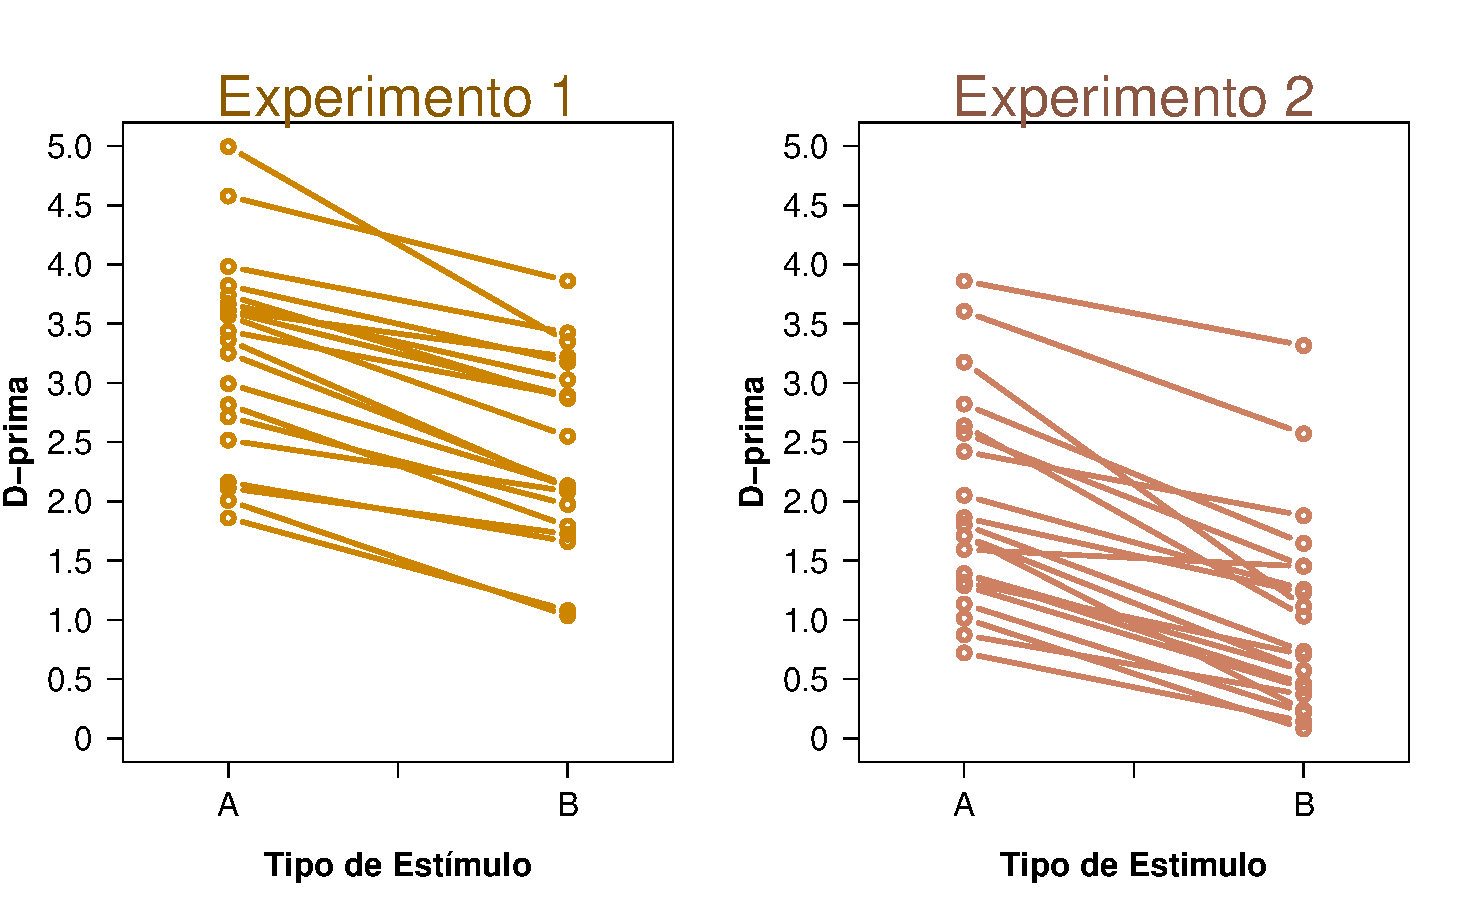
\includegraphics[width=0.80\textwidth]{Figures/Diff_D_E1yE2}
%\decoRule
\caption[Diferencias en Discriminabilidad (Verificando que las condiciones sean, de hecho, diferentes)]{Por cada uno de los experimentos realizados se muestra la relación entre las d' de cada condición de acuerdo a la ejecución de cada uno de los sujetos. En ambos experimentos, se observa una tendencia sistemática a tener mayores niveles de d' en la condición con pocos círculos en las figuras de Ebbinghaus.}
\label{fig:Diff_D}
\end{figure}

\subsection{Análisis 1: Prueba T para comparar las medias de d' por cada condición}

\begin{table}
\caption[Prueba T para evaluar diferencias en las medias de d' entre las condiciones]{Diferencias en d'}
\label{Tabla_t-HitsyFA}
\centering
\begin{tabular}{l | c c c c}
\toprule
%\tabhead{Groups} & \tabhead{Treatment X} & \tabhead{Treatment Y} \\
\textbf{Experimento} & \textbf{$\mu$ A} & \textbf{$\mu$ B} & \textbf{T}  & \textbf{P value}\\
\midrule
Experiment 1 & 3.240 & 2.448 & -3.0587 & 0.0020 \\
Experiment 2 & 1.950 & 1.022 & -3.4972 & 0.0005 \\
\bottomrule
\end{tabular}
\end{table}


\subsection{Análisis 2: Modelo jerárquico bayesiano: Modelo Delta para diferencias en d'}

Se desarrolló un modelo jerárquico bayesiano que asume que las d' y los sesgos C estimados por cada participante en cada una de las condiciones provienen de una distribución normal. El modelo incorpora un parámetro $\delta$ que representa las diferencias entre las medias de las d' estimadas por concidión.

El modelo desarrollado puede verse en la Figura~\ref{fig:Mod_Delta}, estando compuesto por los siguientes elementos:

\begin{itemize}
\item \textbf{Los datos: la materia prima que se señala con nodos sombreados.}
Dado el diseño experimental, conocemos el número total de ensayos con ruido (n) y señal (s). Adicionalmente, por cada participante sabemos cuál es el número total de Hits y Falsas Alarmas cometidos durante el experimento ($H_ij$ y $Fa_ij$, respectivamente). En el modelo, los datos se contienen en nodos cuadrados porque son variables discretas (Nodos circulares indican variables contínuas).\\

\item \textbf{Las tasas como una probabilidad oculta.} 
En la literatura clásica en TDS las tasas de hits y falsas alarmas se interpretan directamente como la proporción de las distribuciones de señal y ruido que caen por encima del criterio ($REFERENCIAS$), respectivamente. Sin embargo, el modelamiento bayesiano nos permite asumir que el número de Hits y Falsas Alarmas observado en cada participante es el resultado de una probabilidad oculta, como parte de un proceso biniomial. Es decir, se asume que el número de Hits y Falsas alarmas

\item \textbf{Sesgo y Discriminabilidad}
De acuerdo con la TDS, las tasas 

\item \textbf{Plato de participantes} 

\item \textbf{Estructura jerárquica:}

\item \textbf{Plato de Condición}

\item \textbf{Parámetro Delta}
\end{itemize} 

\begin{figure}[th]
\centering
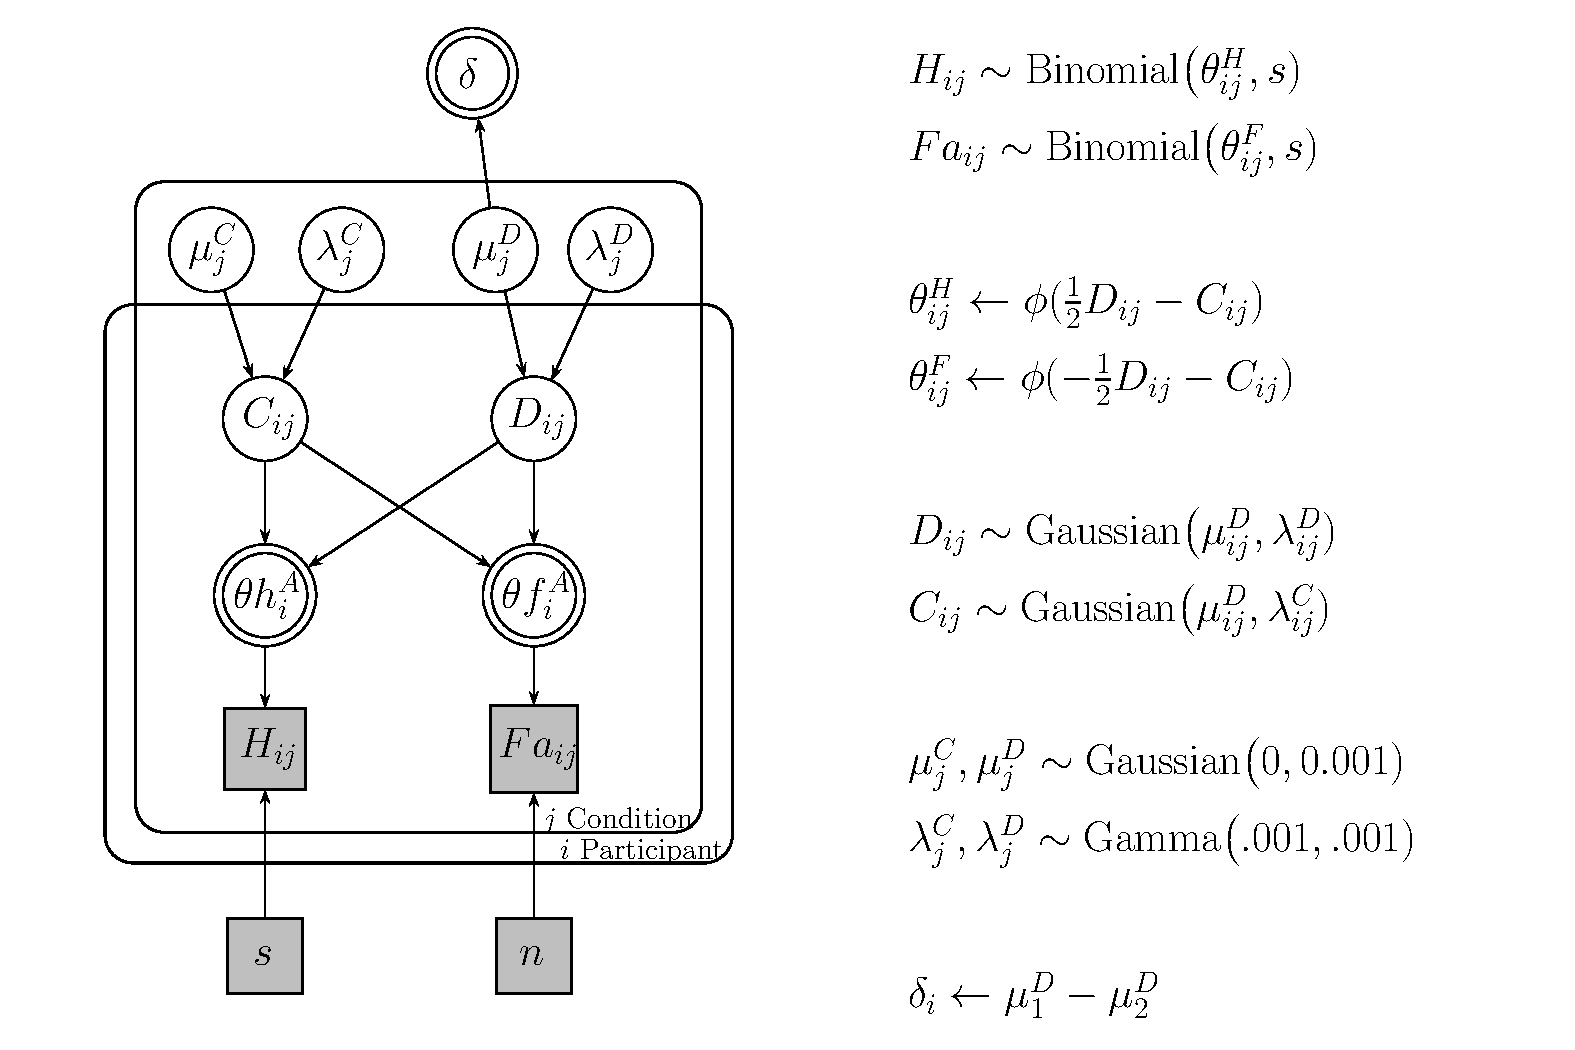
\includegraphics[width=1.1\textwidth]{Figures/Model_Delta_Diff_D}
%\decoRule
\caption[Modelo Delta: Un modelo jerárquico bayesiano para revisar las diferencias en d']{Modelo jerárquico bayesiano con un parámetro Delta ($\delta$) que representa las diferencias en las medias de d' entre las dos condiciones. El modelo tiene priors no informativas.}
\label{fig:Mod_Delta}
\end{figure}









\section{Diferencias en las Tasas de Hits y Falsas Alarmas}

\begin{figure}[th]
\centering
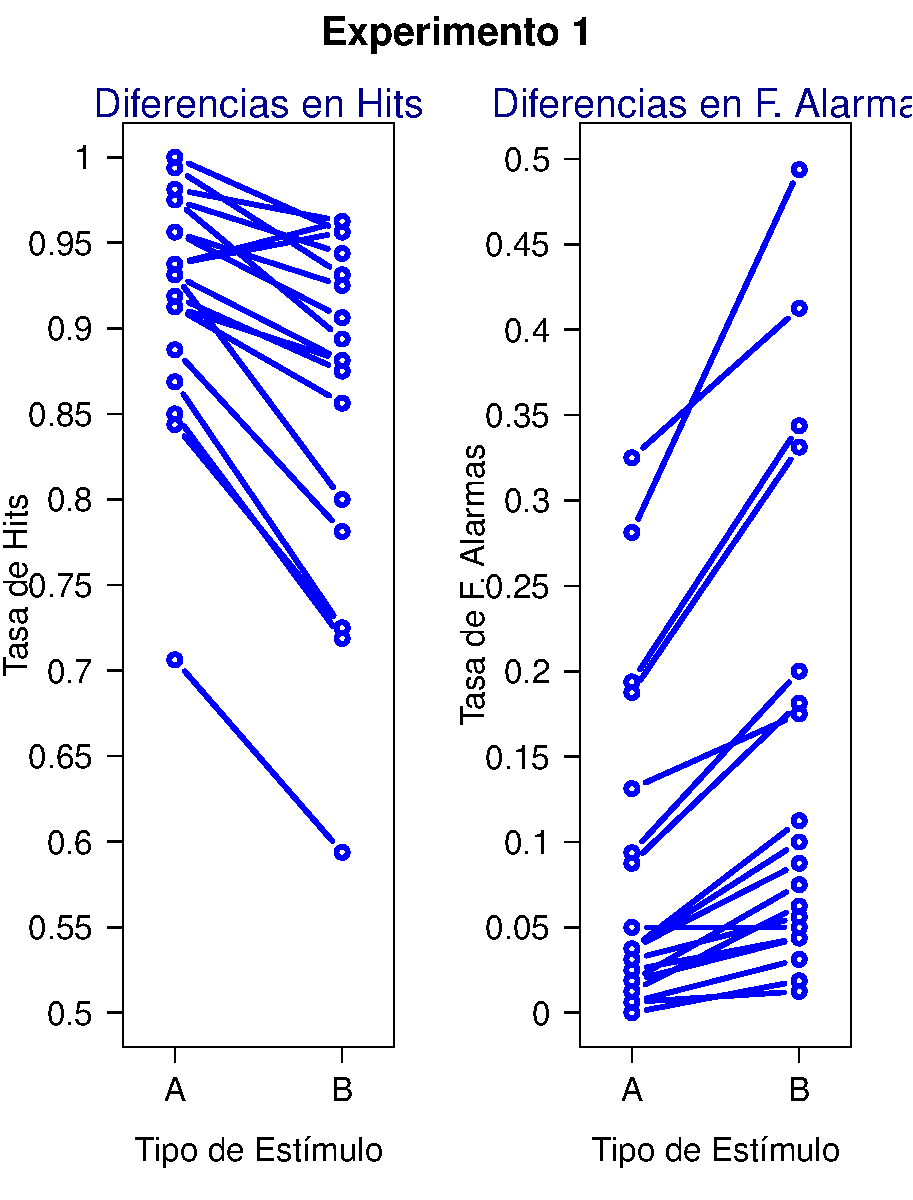
\includegraphics[width=0.80\textwidth]{Figures/Diff_Rate_E1}\\ 
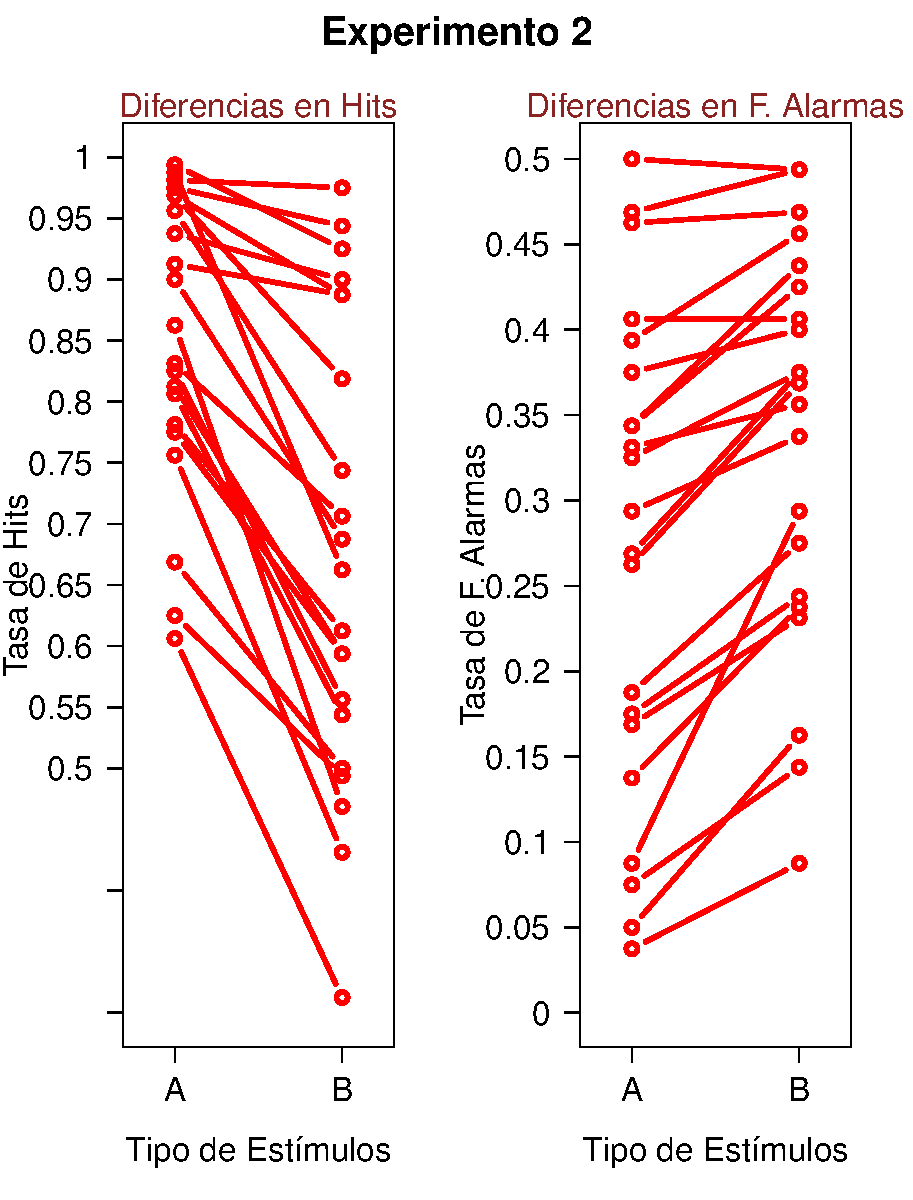
\includegraphics[width=0.80\textwidth]{Figures/Diff_Rate_E2}
%\decoRule
\caption[Diferencias en Tasas (Evaluando diferencias en el desempeño entre las condiciones)]{Comparación intrasujeto de}
\label{fig:Diff_Rate}
\end{figure}


\subsection{Análisis 1: Prueba T}



\begin{table}
\caption[Prueba T para evaluar diferencias en las medias de las tasas de ejecución (Hits y F. Alarmas) entre condiciones]{Diferencias en Hits y Falsas Alarmas entre los tipos de estímulos (Experimento 1 y 2)}
\label{Tabla_t-HitsyFA}
\centering
\begin{tabular}{l l | c c c c}
\toprule
%\tabhead{Groups} & \tabhead{Treatment X} & \tabhead{Treatment Y} \\
\textbf{Experimento} & \textbf{Tasa} & \textbf{$\mu$ A} & \textbf{$\mu$ B} & \textbf{T} & \textbf{P value}\\
\midrule
Exp 1 & Hits & 0.922 & 0.860 & -2.4348 & 0.0098 \\
Exp 1 & FA & 0.08 & 0.143 & 1.917 & 0.0314 \\
Exp 2 & Hits & 0.853 & 0.678 & -3.4757, & 0.0006 \\
Exp 2 & FA & 0.268 & 0.336 & 1.769 & 0.0425 \\
\bottomrule
\end{tabular}
\end{table}


\subsection{Modelo bayesiano}


\begin{figure}[th]
\centering
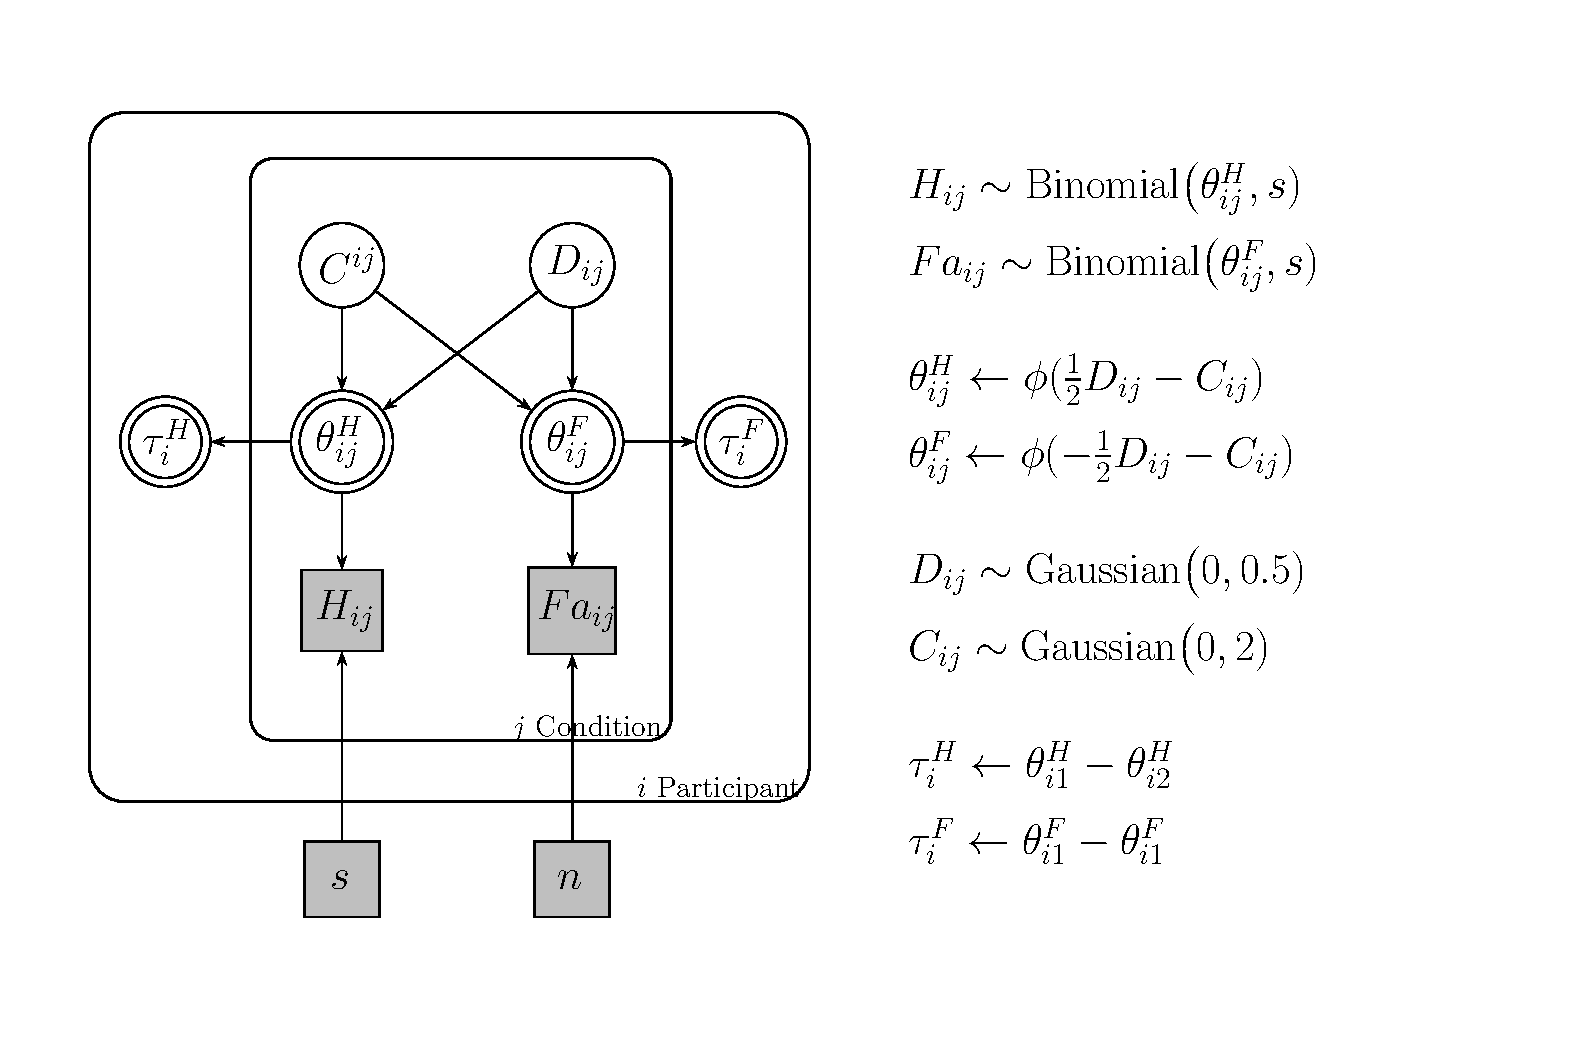
\includegraphics[width=1.1\textwidth]{Figures/Model_Tau_Diff_Tetas}
%\decoRule
\caption[Modelo Tau: Modelo Bayesiano para evaluar las diferencias entre las tasas de hits y falsas alarmas]{Comparación intrasujeto de}
\label{fig:Mod_Tau}
\end{figure}














\section{Diferencias en la asignación de Puntajes de Confianza}

\subsection{Análisis 1: }

\begin{table}
\caption[Prueba T para evaluar diferencias en las medias de los puntajes de confianza asigandos entre condiciones]{}
\label{Tabla_t-HitsyFA}
\centering
\begin{tabular}{l l |  c c c c}
\toprule
%\tabhead{Groups} & \tabhead{Treatment X} & \tabhead{Treatment Y} \\
\textbf{Experimento} & \textbf{Ensayo} & \textbf{$\mu$ A} & \textbf{$\mu$ B} & \textbf{T} & \textbf{P value}\\
\midrule
Exp 1 & Signal & 5.445 & 5.212 & -1.7778, & 0.0418 \\
Exp 1 & Noise & 1.542 & 1.883 & -1.7208 & 0.0472 \\
Exp 2 & Signal & 5.183 & 4.342  & -3.6752, & 0.0004 \\
Exp 2 & Noise & 2.386 & 2.752 & -1.809 & 0.0391 \\
\bottomrule
\end{tabular}
\end{table}












\section{Réplica de controles reportados en la literatura}



